\documentclass[11pt]{article}

%%%%%%%%%%%%%%%%%%%%%%%%%%%%%%%%%%%%%%%%%%%%%%%%%%%%%%%%%%%%%%%%%%%%%%
%\pdfminorversion=4
% NOTE: To produce blinded version, replace "0" with "1" below.
\newcommand{\blind}{0}

%%%%%%% IISE Transactions margin specifications %%%%%%%%%%%%%%%%%%%
\addtolength{\oddsidemargin}{-.5in}%
\addtolength{\evensidemargin}{-.5in}%
\addtolength{\textwidth}{1in}%
\addtolength{\textheight}{1.3in}%
\addtolength{\topmargin}{-.8in}%

\makeatletter
\renewcommand\section{\@startsection {section}{1}{\z@}%
	{-3.5ex \@plus -1ex \@minus -.2ex}%
	{2.3ex \@plus.2ex}%
	{\normalfont\fontfamily{phv}\fontsize{16}{19}\bfseries}}
\renewcommand\subsection{\@startsection{subsection}{2}{\z@}%
	{-3.25ex\@plus -1ex \@minus -.2ex}%
	{1.5ex \@plus .2ex}%
	{\normalfont\fontfamily{phv}\fontsize{14}{17}\bfseries}}
\renewcommand\subsubsection{\@startsection{subsubsection}{3}{\z@}%
	{-3.25ex\@plus -1ex \@minus -.2ex}%
	{1.5ex \@plus .2ex}%
	{\normalfont\normalsize\fontfamily{phv}\fontsize{14}{17}\selectfont}}
\makeatother
%%%%%%%%%%%%%%%%%%%%%%%%%%%%%%%%%%%%%%%%%%%%%%%%%%%%%%%%%%%%%%%%%%%%%%%%%

%%%%% IISE Transactions package list %%%%%%%%%%%%%%%%%%%%%%%%%%%%%%%%%%%%%%
	\usepackage{amsmath}
	\usepackage[UTF8, heading=false]{ctex} % [#4/#5] Ensure Chinese captions and supplementary notes render correctly.
	\usepackage{graphicx}
\usepackage{enumerate}
\usepackage{natbib}
\usepackage{url}
\usepackage{xcolor}
\usepackage{enumitem}
\usepackage{amssymb}
\usepackage{algorithm}
\usepackage{algpseudocode}
\usepackage{bm}
\usepackage{setspace}
\usepackage{float}
\usepackage{subcaption}
\usepackage{booktabs}
\usepackage{multirow}

\begin{document}

	%%%%%%%%%%%%%%%%%%%%%%%%%%%%%%%%%%%%%%%%%%%%%%%%%%%%%%%%%%%%%%%%%%%%%%%%%%%%%%
	\def\spacingset#1{\renewcommand{\baselinestretch}%
		{#1}\small\normalsize} \spacingset{1}
	%%%%%%%%%%%%%%%%%%%%%%%%%%%%%%%%%%%%%%%%%%%%%%%%%%%%%%%%%%%%%%%%%%%%%%%%%%%%%%

	% =========================================================================
	%                           单独文件的标题页设置
	% =========================================================================

	\if0\blind
	{
		\begin{center}
			% 标题：明确指出是补充材料
			{\LARGE \bfseries Supplementary Materials for: \\[\baselineskip]
				``Dual-Attention Deep Gaussian Processes for Multi-Objective Robust Parameter Design''}

			\vspace{0.8cm} % 间距

			% 作者信息

		\end{center}
	} \fi

	\if1\blind
	{
		\bigskip
		\begin{center}
			{\LARGE \bfseries Supplementary Materials for: \\[\baselineskip]
				``Dual-Attention Deep Gaussian Processes for Multi-Objective Robust Parameter Design''}
		\end{center}
		\medskip
	} \fi

	\bigskip
	\bigskip

	% =========================================================================
	%                           附录内容设置
	% =========================================================================

	\appendix % 将后续 Section 编号改为 A, B, C...

	% --- 设置公式、图表的编号格式为 A.1, B.1 等 ---
	\renewcommand{\theequation}{\Alph{section}.\arabic{equation}}
	\renewcommand{\thefigure}{\Alph{section}.\arabic{figure}}
	\renewcommand{\thetable}{\Alph{section}.\arabic{table}}
	\newcommand{\resetappendixcounters}{%
		\setcounter{equation}{0}%
		\setcounter{figure}{0}%
		\setcounter{table}{0}%
	}
	\resetappendixcounters % [#1]

	% ---------------- Appendix A ----------------
	% 您可以在这里修改标题，例如 "Proofs" 或 "Mathematical Derivations"
	\section{Derivation of the Variational ELBO for Sparse GPs} \label{app:A}
	\resetappendixcounters % [#1] Ensure equations, figures, and tables start from A.1.

	This appendix provides a detailed derivation of the Evidence Lower Bound (ELBO) (Equation 4) described in Section 2.2. We consider the augmented GP model by introducing $M$ inducing points $\mathbf{Z}$ and corresponding inducing variables $\mathbf{u}$. The joint probability of the observations $\mathbf{y}$, latent functions $\mathbf{f}$, and inducing variables $\mathbf{u}$ is given by:
	\begin{equation}
		p({\bf{y}},{\bf{f}},{\bf{u}}) = p({\bf{y}}|{\bf{f}})p({\bf{f}}|{\bf{u}})p({\bf{u}}),
	\end{equation}
	where $p(\mathbf{u}) = \mathcal{N}(\mathbf{0}, \mathbf{K}_{\mathbf{uu}})$ is the prior over inducing variables, and $p(\mathbf{f} | \mathbf{u})$ follows the standard GP conditional distribution. To approximate the intractable posterior $p(\mathbf{f}, \mathbf{u} | \mathbf{y})$, we propose a variational distribution $q(\mathbf{f}, \mathbf{u})$. Following the framework of Titsias (2009), we enforce the variational posterior to factorize as:
	\begin{equation}
		q({\bf{f}},{\bf{u}}) = p({\bf{f}}|{\bf{u}})q({\bf{u}}),
	\end{equation}
	where $q(\mathbf{u}) = \mathcal{N}(\mathbf{m}, \mathbf{S})$ is a free variational distribution to be optimized, and $p(\mathbf{f} | \mathbf{u})$ is fixed to the model prior conditionals. This corresponds to Equation (4) in the main text. \textcolor{red}{The goal} of variational inference is to minimize the Kullback-Leibler (KL) divergence between the approximate posterior and the true posterior, which is equivalent to maximizing the ELBO:% [#3]
	\begin{equation}
		\mathcal{L} = \iint q(\mathbf{f}, \mathbf{u}) \log \frac{p(\mathbf{y}, \mathbf{f}, \mathbf{u})}{q(\mathbf{f}, \mathbf{u})} \, d\mathbf{f} d\mathbf{u}
	\end{equation}

	Substituting (A.1) and (A.2) into (A.3), the ELBO can be expanded as:
	\begin{equation}
		\begin{aligned}
			\mathcal{L} &= \iint p(\mathbf{f}|\mathbf{u})q(\mathbf{u}) \log \frac{p(\mathbf{y}|\mathbf{f})p(\mathbf{f}|\mathbf{u})p(\mathbf{u})}{p(\mathbf{f}|\mathbf{u})q(\mathbf{u})} \, d\mathbf{f}d\mathbf{u} \\
			&= \iint p(\mathbf{f}|\mathbf{u})q(\mathbf{u}) \left[ \log p(\mathbf{y}|\mathbf{f}) + \log \frac{p(\mathbf{u})}{q(\mathbf{u})} \right] \, d\mathbf{f}d\mathbf{u}
		\end{aligned}.
	\end{equation}

	The term $p(\mathbf{f} | \mathbf{u})$ cancels out in the logarithm ratio, significantly simplifying the computation. The equation splits into two components:

	(1) Expected Log-Likelihood:
	\begin{equation}
		\iint q(\mathbf{u})\,p(\mathbf{f}\mid \mathbf{u})\,\log p(\mathbf{y}\mid \mathbf{f})\,d\mathbf{f}\,d\mathbf{u}
		= \mathbb{E}_{q(\mathbf{f})}\!\left[\log p(\mathbf{y}\mid \mathbf{f})\right]
		= \sum_{i=1}^{N}\mathbb{E}_{q(f_i)}\!\left[\log p(y_i\mid f_i)\right],
	\end{equation}
	where $q(\mathbf{f}) = \int p(\mathbf{f} | \mathbf{u}) q(\mathbf{u}) d\mathbf{u}$ represents the marginal variational distribution.

	(2) KL Divergence:
	\begin{equation}
		\int q(\mathbf{u})\left[\int p(\mathbf{f}\mid \mathbf{u})\,d\mathbf{f}\right]
		\log\frac{p(\mathbf{u})}{q(\mathbf{u})}\,d\mathbf{u}
		= -\mathrm{KL}\!\left[q(\mathbf{u})\,\|\,p(\mathbf{u})\right].
	\end{equation}
	Note that $\int p(\mathbf{f} | \mathbf{u}) d\mathbf{f} = 1$.
	Combining (A.5) and (A.6), we obtain the final ELBO formulation as presented in Equation (4):
	\begin{equation}
		\mathcal{L}_{\mathrm{SGP}}
		= \sum_{i=1}^{N}\mathbb{E}_{q(f_i)}\!\left[\log p(y_i\mid f_i)\right]
		- \mathrm{KL}\!\left[q(\mathbf{u})\,\|\,p(\mathbf{u})\right].
	\end{equation}










	% ---------------- Appendix B ----------------
	% 您可以在这里修改标题，例如 "Additional Experiments"
	\section{Proof of Unbiased Gradient Estimation via Reparameterization Trick} \label{app:B}
	\resetappendixcounters % [#1]

	This appendix provides the mathematical justification for the gradient computation in the Doubly Stochastic Variational Inference (DSVI) framework, specifically concerning Equations (9)-(12) in Section 2.3.
	We aim to compute the gradient of the expected log-likelihood term in the ELBO with respect to the variational parameters $\boldsymbol{\phi}$ (i.e., $\mathbf{m}, \mathbf{S}$). The objective function is:
	\begin{equation}
		\mathcal{L}(\phi)
		= \mathbb{E}_{q_{\phi}(\mathbf{f})}\!\left[\log p(\mathbf{y}\mid \mathbf{f})\right]
		= \int q_{\phi}(\mathbf{f})\,\log p(\mathbf{y}\mid \mathbf{f})\,d\mathbf{f}.
	\end{equation}
	Directly differentiating (B.1) is problematic because the integration domain depends on $\boldsymbol{\phi}$. To resolve this, we apply the reparameterization trick defined in Equation (11):
	\begin{equation}
		\mathbf{f}
		= g(\phi,\boldsymbol{\epsilon})
		= \boldsymbol{\mu}_{\phi} + \boldsymbol{\Sigma}_{\phi}^{1/2}\odot \boldsymbol{\epsilon},
		\qquad
		\boldsymbol{\epsilon}\sim p(\boldsymbol{\epsilon})=\mathcal{N}(\mathbf{0},\mathbf{I}).
	\end{equation}
	Using the Law of the Unconscious Statistician (LOTUS), the expectation over $q_{\boldsymbol{\phi}}(\mathbf{f})$ can be rewritten as an expectation over the auxiliary noise distribution $p(\boldsymbol{\epsilon})$, which is independent of $\boldsymbol{\phi}$:
	\begin{equation}
		\mathcal{L}(\phi)
		= \mathbb{E}_{p(\boldsymbol{\epsilon})}\!\left[\log p\!\left(\mathbf{y}\mid g(\phi,\boldsymbol{\epsilon})\right)\right].
	\end{equation}
	Now, the gradient operator $\nabla_{\boldsymbol{\phi}}$ can be moved inside the expectation:
	\begin{equation}
		\nabla_{\phi}\mathcal{L}(\phi)
		= \nabla_{\phi}\int p(\boldsymbol{\epsilon})\,\log p\!\left(\mathbf{y}\mid g(\phi,\boldsymbol{\epsilon})\right)\,d\boldsymbol{\epsilon}
		= \mathbb{E}_{p(\boldsymbol{\epsilon})}\!\left[\nabla_{\phi}\log p\!\left(\mathbf{y}\mid g(\phi,\boldsymbol{\epsilon})\right)\right].
	\end{equation}
	This expectation can be efficiently approximated using Monte Carlo sampling. For $S$ samples of $\boldsymbol{\epsilon}_s \sim \mathcal{N}(\mathbf{0}, \mathbf{I})$:
	\begin{equation}
		\nabla_{\phi}\mathcal{L}(\phi)
		\approx \frac{1}{S}\sum_{s=1}^{S}\nabla_{\phi}\log p\!\left(\mathbf{y}\mid g(\phi,\boldsymbol{\epsilon}_s)\right).
	\end{equation}
	Since $g(\boldsymbol{\phi}, \boldsymbol{\epsilon})$ is a deterministic differentiable function, the gradients can be computed via standard backpropagation (chain rule). This proves that the reparameterization trick provides an unbiased low-variance gradient estimator for optimizing the ELBO in Equation (9).


	% ---------------- Appendix C ----------------
	% 您可以在这里修改标题，例如 "Sensitivity Analysis"
	\section{Theoretical Justification of the Weighted ELBO} \label{app:C}
	\resetappendixcounters % [#1]

	This appendix provides the theoretical basis for the sample-weighted ELBO objective function defined in Equation (16). \textcolor{red}{Standard} variational inference minimizes the KL divergence between the variational posterior $q(\mathbf{u})$ and the true Bayesian posterior $p(\mathbf{u}|\mathbf{y}) \propto p(\mathbf{y}|\mathbf{f})p(\mathbf{f}|\mathbf{u})p(\mathbf{u})$. This is equivalent to maximizing the standard ELBO:% [#3]
	\begin{equation}
		\mathcal{L}
		= \mathbb{E}_{q}\!\left[\log p(\mathbf{y}\mid \mathbf{f})\right]
		- \mathrm{KL}\!\left[q(\mathbf{u})\,\|\,p(\mathbf{u})\right].
	\end{equation}
	To incorporate the sample-level attention mechanism rigorously, we adopt the framework of generalized variational inference (Knoblauch et al., 2019). In GVI, the standard Bayesian inference is generalized as an optimization problem involving a loss function $\ell$, a divergence $D$, and a prior $\pi$:
	\begin{equation}
		q^{\ast}
		= \arg\min_{q}\left\{\mathbb{E}_{q}\!\left[\ell(\mathbf{y},\mathbf{f})\right] + D\!\left(q\,\|\,\pi\right)\right\}.
	\end{equation}
	In our DA-DGP framework, we define a weighted log-likelihood loss to emphasize the ROI:
	\begin{equation}
		\ell_{\mathrm{weighted}}(\mathbf{y},\mathbf{f})
		= -\sum_{k=1}^{p}\sum_{i=1}^{N}\tilde{s}_{i,k}\,\log p\!\left(y_{i,k}\mid f^{L}_{i,k}\right),
	\end{equation}
	where $\tilde{s}_{i,k}$ are the normalized attention weights derived in Equation (14). Setting the divergence $D$ to be the KL divergence, the optimization objective becomes:
	\begin{equation}
		\mathcal{L}_{\mathrm{DA\text{-}DGP}}
		= \sum_{k=1}^{p}\sum_{i=1}^{N}\tilde{s}_{i,k}\,
		\mathbb{E}_{q(f^{L}_{i,k})}\!\left[\log p\!\left(y_{i,k}\mid f^{L}_{i,k}\right)\right]
		- \mathrm{KL}\!\left[q(\mathbf{u})\,\|\,p(\mathbf{u})\right].
	\end{equation}
	This derivation confirms that our weighted objective (Equation 16) is not merely a heuristic modification but a valid GVI posterior approximation that minimizes a preference-weighted risk bound.

	\newpage
	\section{Supplementary Visualizations of Experimental Results} \label{app:D}
	\resetappendixcounters % [#1]


	\begin{figure}[htbp]
		\centering

		% --- 第一行: Task 1 (a) ---
		\begin{subfigure}[b]{1.0\textwidth}
				\centering
				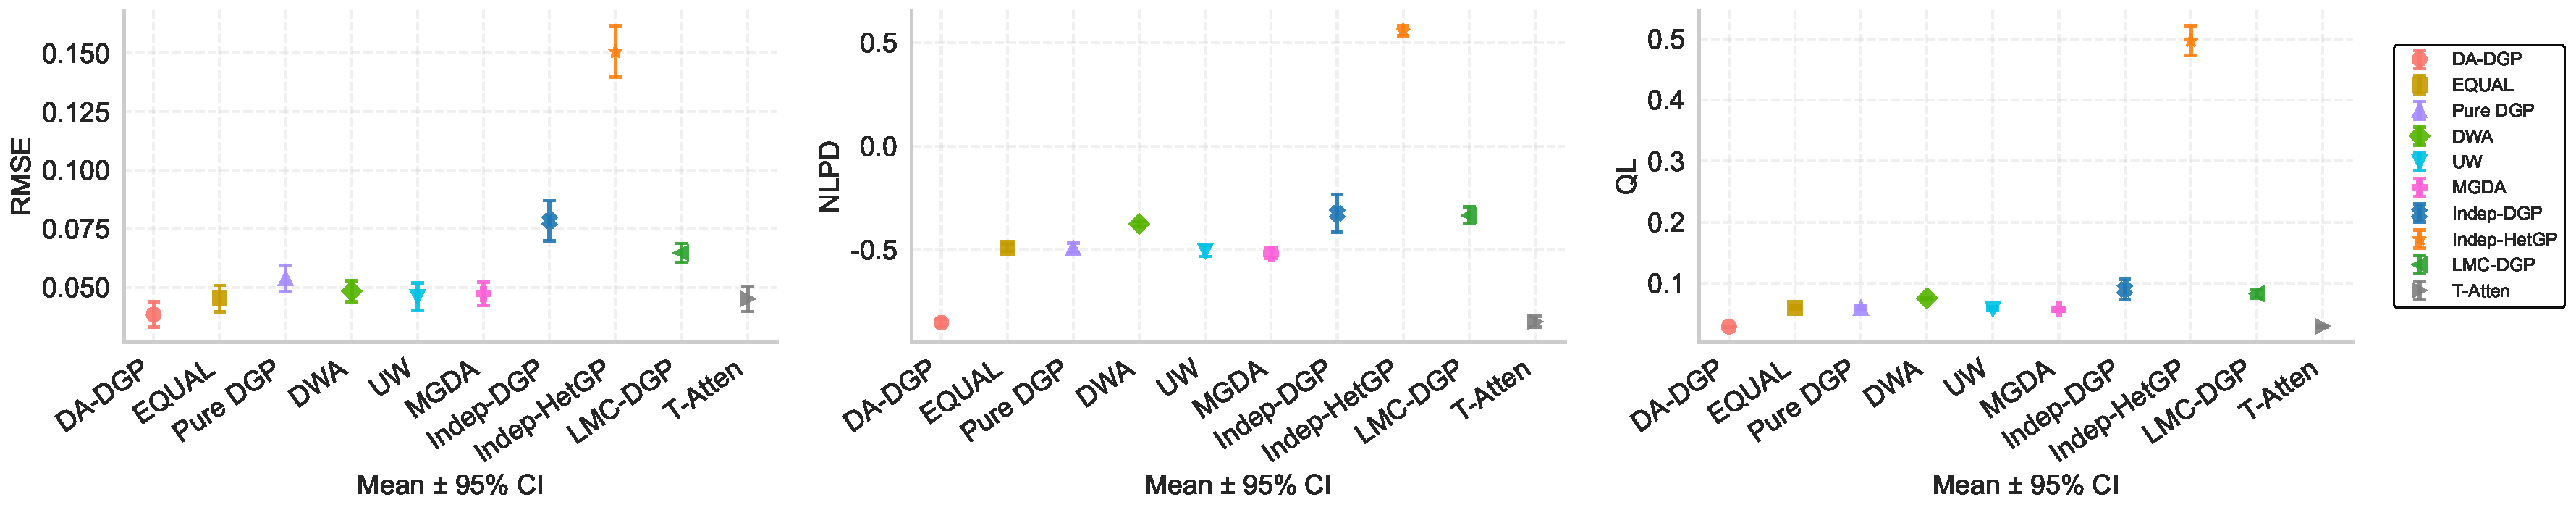
\includegraphics[width=0.8\textwidth]{../mathexam/fig/metrics/task1_metrics.pdf}
				\caption{Task 1 ($y_1$)}
				\label{fig:task1_curves}
			\end{subfigure}

	%	\vspace{0.4cm} % 增加行间距，防止图挨得太近

		% --- 第二行: Task 2 (b) ---
		\begin{subfigure}[b]{1.0\textwidth}
				\centering
				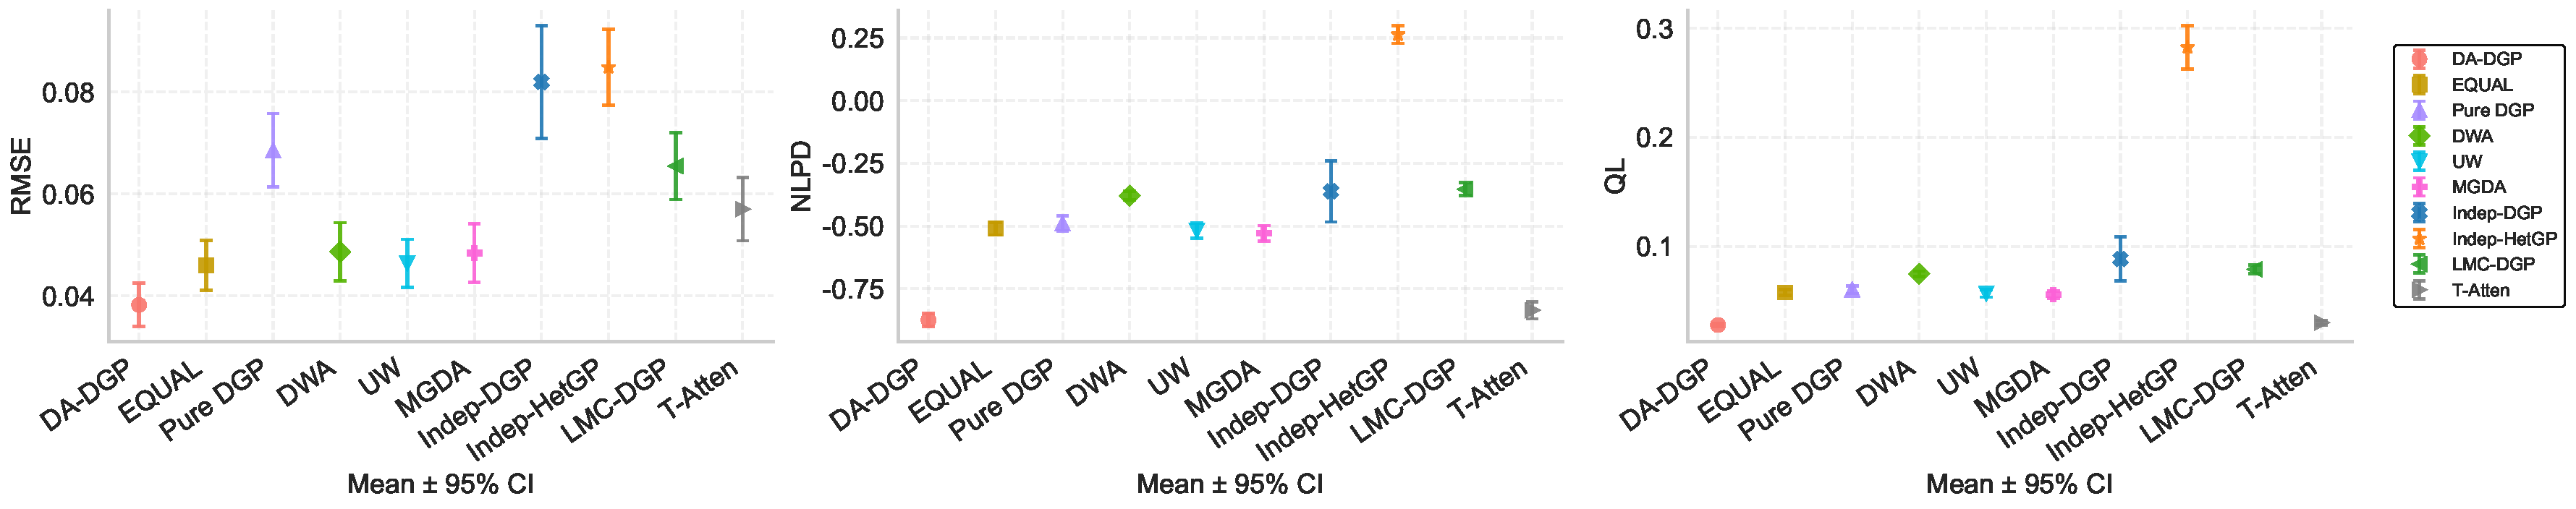
\includegraphics[width=0.8\textwidth]{../mathexam/fig/metrics/task2_metrics.pdf}
				\caption{Task 2 ($y_2$)}
				\label{fig:task2_curves}
			\end{subfigure}

	%	\vspace{0.4cm} % 增加行间距

		% --- 第三行: Task 3 (c) ---
		\begin{subfigure}[b]{1.0\textwidth}
				\centering
				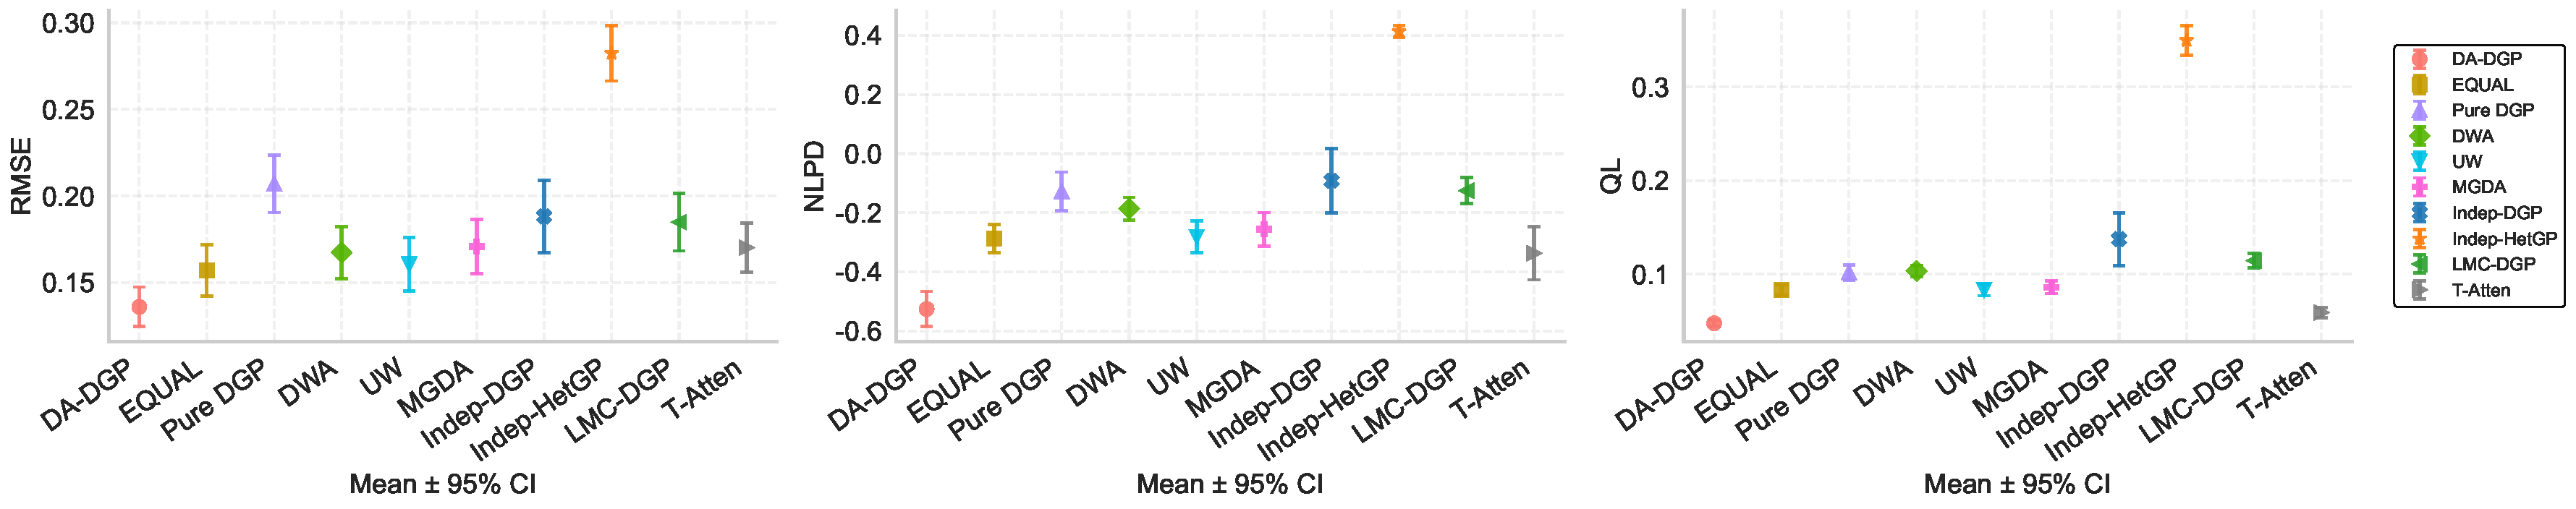
\includegraphics[width=0.8\textwidth]{../mathexam/fig/metrics/task3_metrics.pdf}
				\caption{Task 3 ($y_3$)}
				\label{fig:task3_curves}
			\end{subfigure}

		\caption{\textcolor{red}{Auxiliary taskwise performance metric curves for the numerical example.}}% [#5]
		\caption*{\textcolor{red}{数值算例的辅助分任务性能指标曲线。}}% [#5]
		\label{fig:performance_curves}
	\end{figure}

	\newpage
	\section{Sensitivity Analyses for the Numerical Example} \label{app:E}
	\resetappendixcounters % [#1]

	This appendix reports the detailed sensitivity analyses referenced in Section 4.1 of the main paper. We consider three factors: the Gaussian bandwidth used in sample-level attention, the surrogate depth/hidden complexity, and the available training sample size. All statistics are aggregated over 20 independent runs, and the figures below visualize taskwise error bars for RMSE, NLPD, and QL.

	本附录给出正文 Section 4.1 引用的详细敏感性分析结果。我们考察三个因素：样本级注意力中的 Gaussian bandwidth、代理模型的深度/隐藏复杂度，以及可用训练样本量。所有统计量均基于 20 次独立运行汇总得到，下列图表进一步展示了各任务在 RMSE、NLPD 和 QL 上的误差棒结果。

	\subsection{Bandwidth Sensitivity} \label{app:E1}
	The bandwidth study confirms that moderate kernels are preferable. Averaged over three tasks, $\sigma=0.5$ yields the best QL (\textbf{0.034774}), while $\sigma=0.3$ attains the best RMSE (\textbf{0.069403}) and remains very close to $\sigma=0.5$. In contrast, $\sigma=0.1$ degrades both RMSE and QL, indicating over-localization of the training signal. Hence, the default choice $\sigma=0.5$ provides the most balanced overall behavior.

	带宽敏感性结果表明，中等带宽更为合适。在三个任务平均意义下，$\sigma=0.5$ 取得最佳 QL（\textbf{0.034774}），而 $\sigma=0.3$ 取得最佳 RMSE（\textbf{0.069403}），且与 $\sigma=0.5$ 非常接近。相比之下，$\sigma=0.1$ 会同时恶化 RMSE 和 QL，说明训练信号被过度局部化。因此，默认设定 $\sigma=0.5$ 在综合表现上最为均衡。

	\begin{table}[htbp]
		\centering
		\caption{Average sensitivity summary for Gaussian bandwidth.}
		\caption*{Gaussian 带宽的平均敏感性汇总。}
		\label{tab:sigma_sensitivity_avg}
		\begin{tabular}{lccc}
			\toprule
			Condition & Avg. RMSE & Avg. NLPD & Avg. QL \\
			\midrule
			$\sigma=0.1$ & 0.090653 & -0.611964 & 0.044973 \\
			$\sigma=0.3$ & \textbf{0.069403} & -0.734488 & 0.035847 \\
			$\sigma=0.5$ & 0.070831 & \textbf{-0.750523} & \textbf{0.034774} \\
			$\sigma=0.7$ & 0.075690 & -0.737188 & 0.035506 \\
			$\sigma=1.0$ & 0.078762 & -0.731904 & 0.035760 \\
			$\sigma=1.5$ & 0.082363 & -0.717340 & 0.036645 \\
			\bottomrule
		\end{tabular}
	\end{table}

	\begin{figure}[htbp]
		\centering
		\begin{subfigure}[b]{0.9\textwidth}
			\centering
			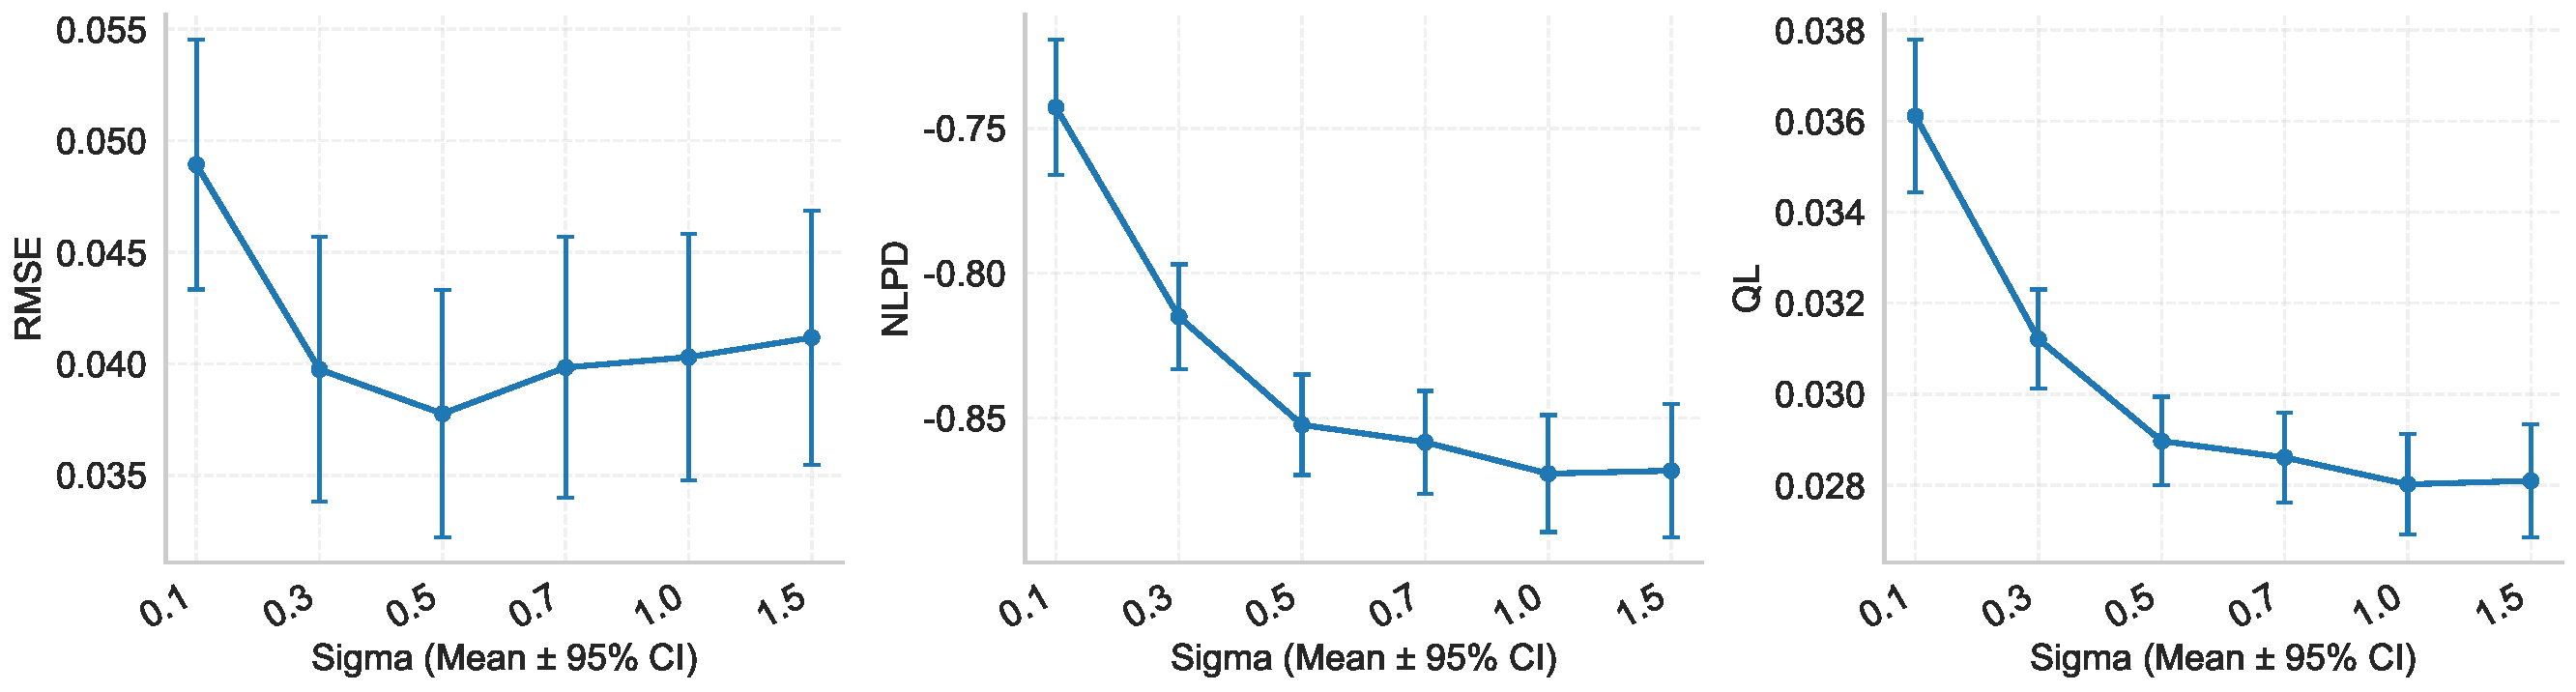
\includegraphics[width=\textwidth]{../mathexam/fig/sensitivity/sigma_sensitivity/task1_metrics_errorbars.pdf}
			\caption{Task 1}
		\end{subfigure}

		\begin{subfigure}[b]{0.9\textwidth}
			\centering
			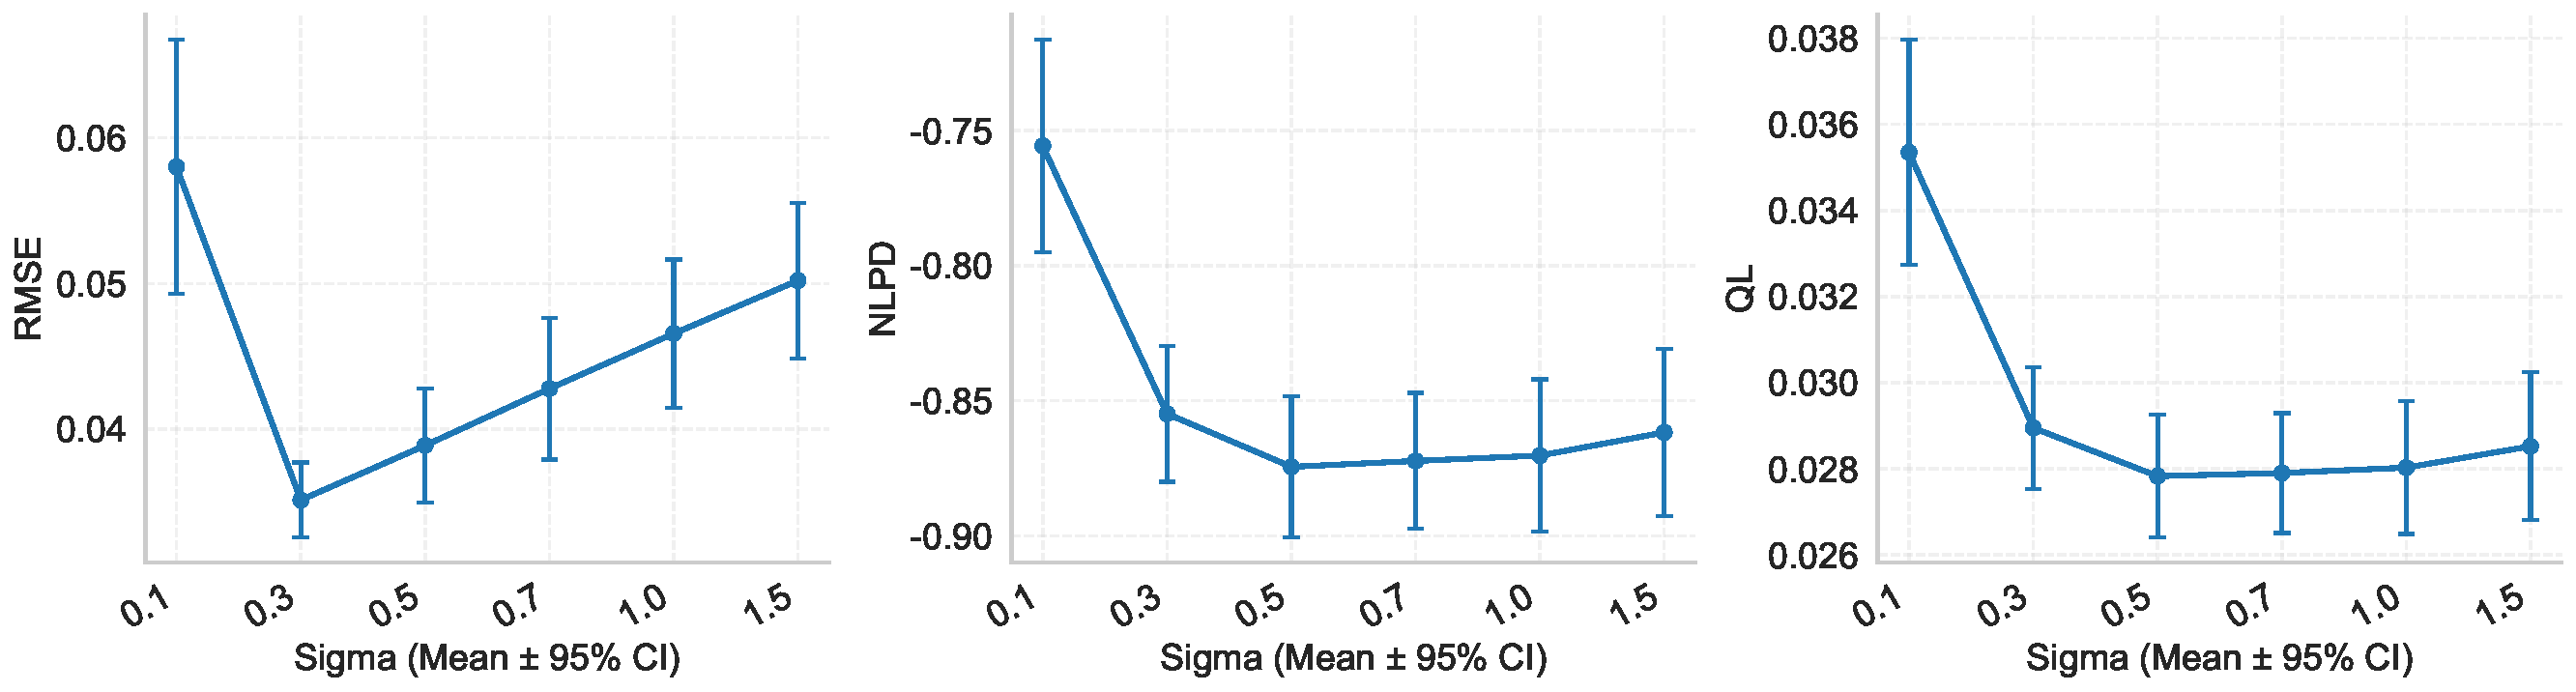
\includegraphics[width=\textwidth]{../mathexam/fig/sensitivity/sigma_sensitivity/task2_metrics_errorbars.pdf}
			\caption{Task 2}
		\end{subfigure}

		\begin{subfigure}[b]{0.9\textwidth}
			\centering
			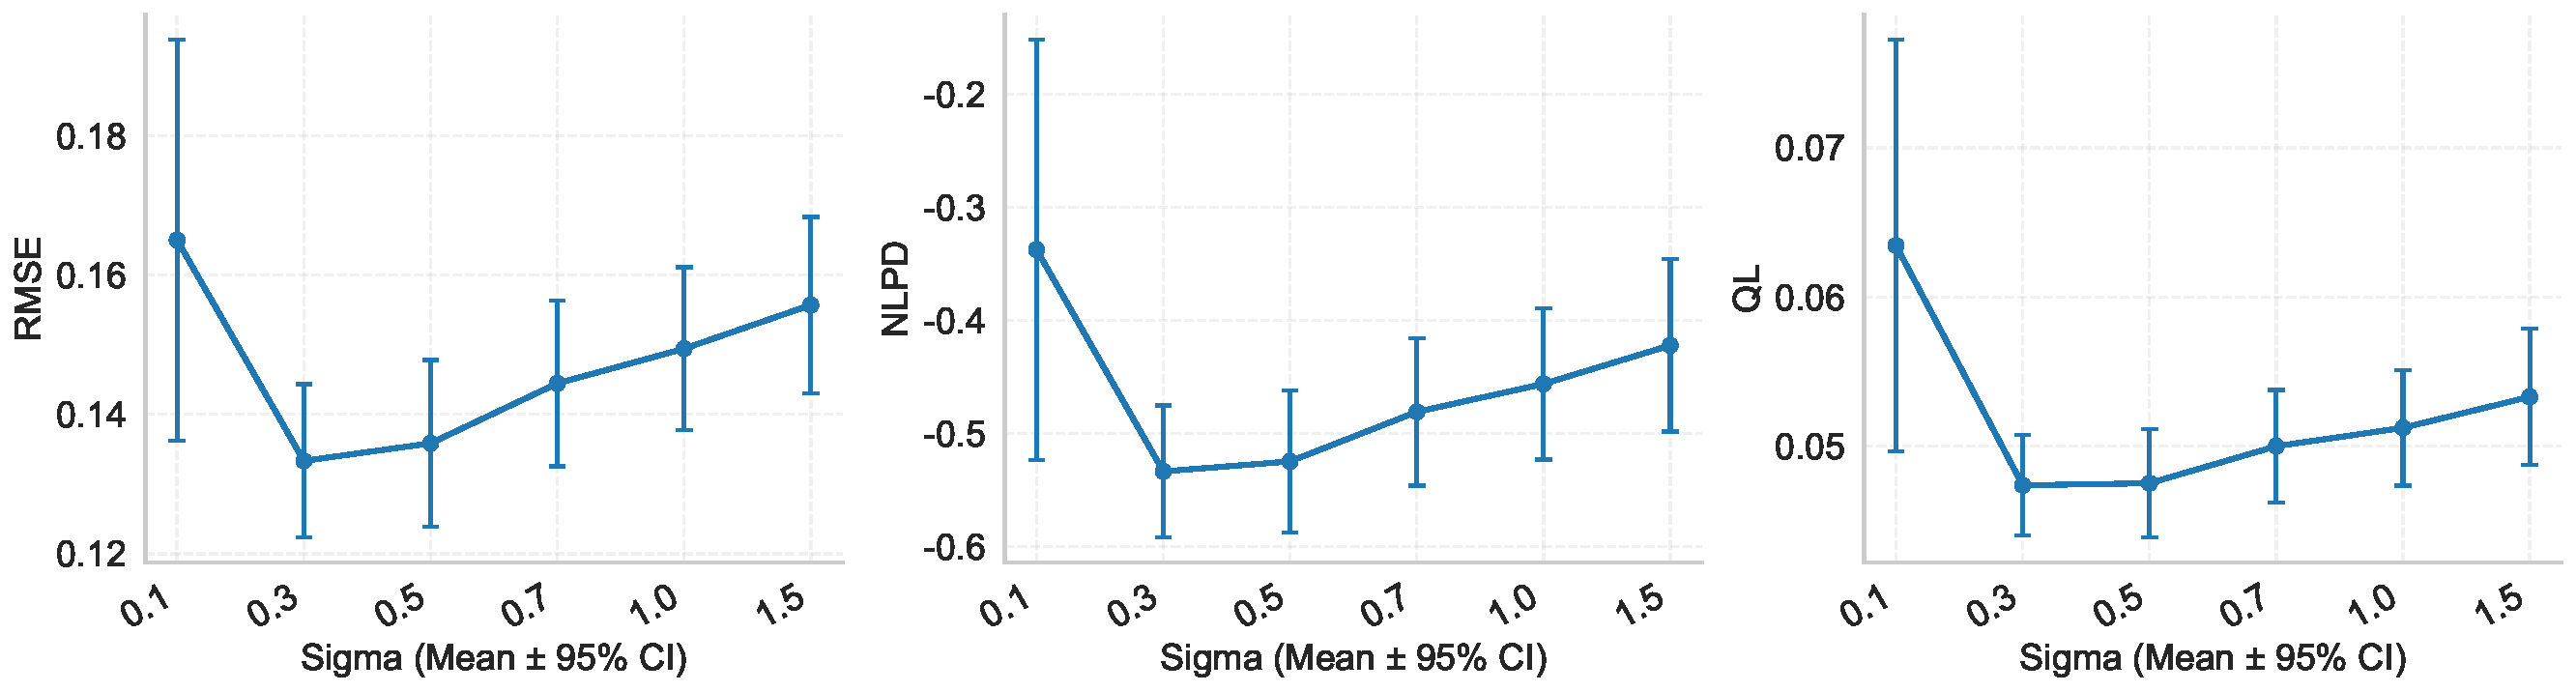
\includegraphics[width=\textwidth]{../mathexam/fig/sensitivity/sigma_sensitivity/task3_metrics_errorbars.pdf}
			\caption{Task 3}
		\end{subfigure}
		\caption{Taskwise error-bar plots for Gaussian bandwidth sensitivity.}
		\caption*{Gaussian 带宽敏感性的分任务误差棒图。}
		\label{fig:sigma_sensitivity}
	\end{figure}

	\subsection{Depth and Hidden Complexity Sensitivity} \label{app:E2}
	The depth study shows that the default configuration is not only simpler but also clearly superior. The 2L-D5 model achieves the best average RMSE (\textbf{0.070808}), NLPD (\textbf{-0.751518}), and QL (\textbf{0.034732}). Shallower 2L-D2 underfits, while deeper 3L-D5, 4L-D5, and 5L-D5 rapidly deteriorate, suggesting that the current 5-dimensional benchmark with 400 training samples does not benefit from additional depth.

	深度与隐藏复杂度敏感性表明，默认配置不仅更简单，而且性能也显著更优。2L-D5 在平均 RMSE（\textbf{0.070808}）、NLPD（\textbf{-0.751518}）和 QL（\textbf{0.034732}）上均为最佳。较浅的 2L-D2 存在欠拟合，而更深的 3L-D5、4L-D5 和 5L-D5 则迅速恶化，说明当前 5 维、400 样本的基准问题并不能从额外深度中获益。

	\begin{table}[htbp]
		\centering
		\caption{Average sensitivity summary for depth and hidden complexity.}
		\caption*{深度与隐藏复杂度的平均敏感性汇总。}
		\label{tab:depth_sensitivity_avg}
		\begin{tabular}{lccc}
			\toprule
			Condition & Avg. RMSE & Avg. NLPD & Avg. QL \\
			\midrule
			2L-D2 & 0.246244 & 0.084328 & 0.185969 \\
			2L-D5 & \textbf{0.070808} & \textbf{-0.751518} & \textbf{0.034732} \\
			3L-D5 & 0.291672 & 0.405546 & 0.282074 \\
			4L-D5 & 0.460090 & 0.774311 & 0.650473 \\
			5L-D5 & 0.706363 & 1.235559 & 1.192501 \\
			\bottomrule
		\end{tabular}
	\end{table}

	\begin{figure}[htbp]
		\centering
		\begin{subfigure}[b]{0.9\textwidth}
			\centering
			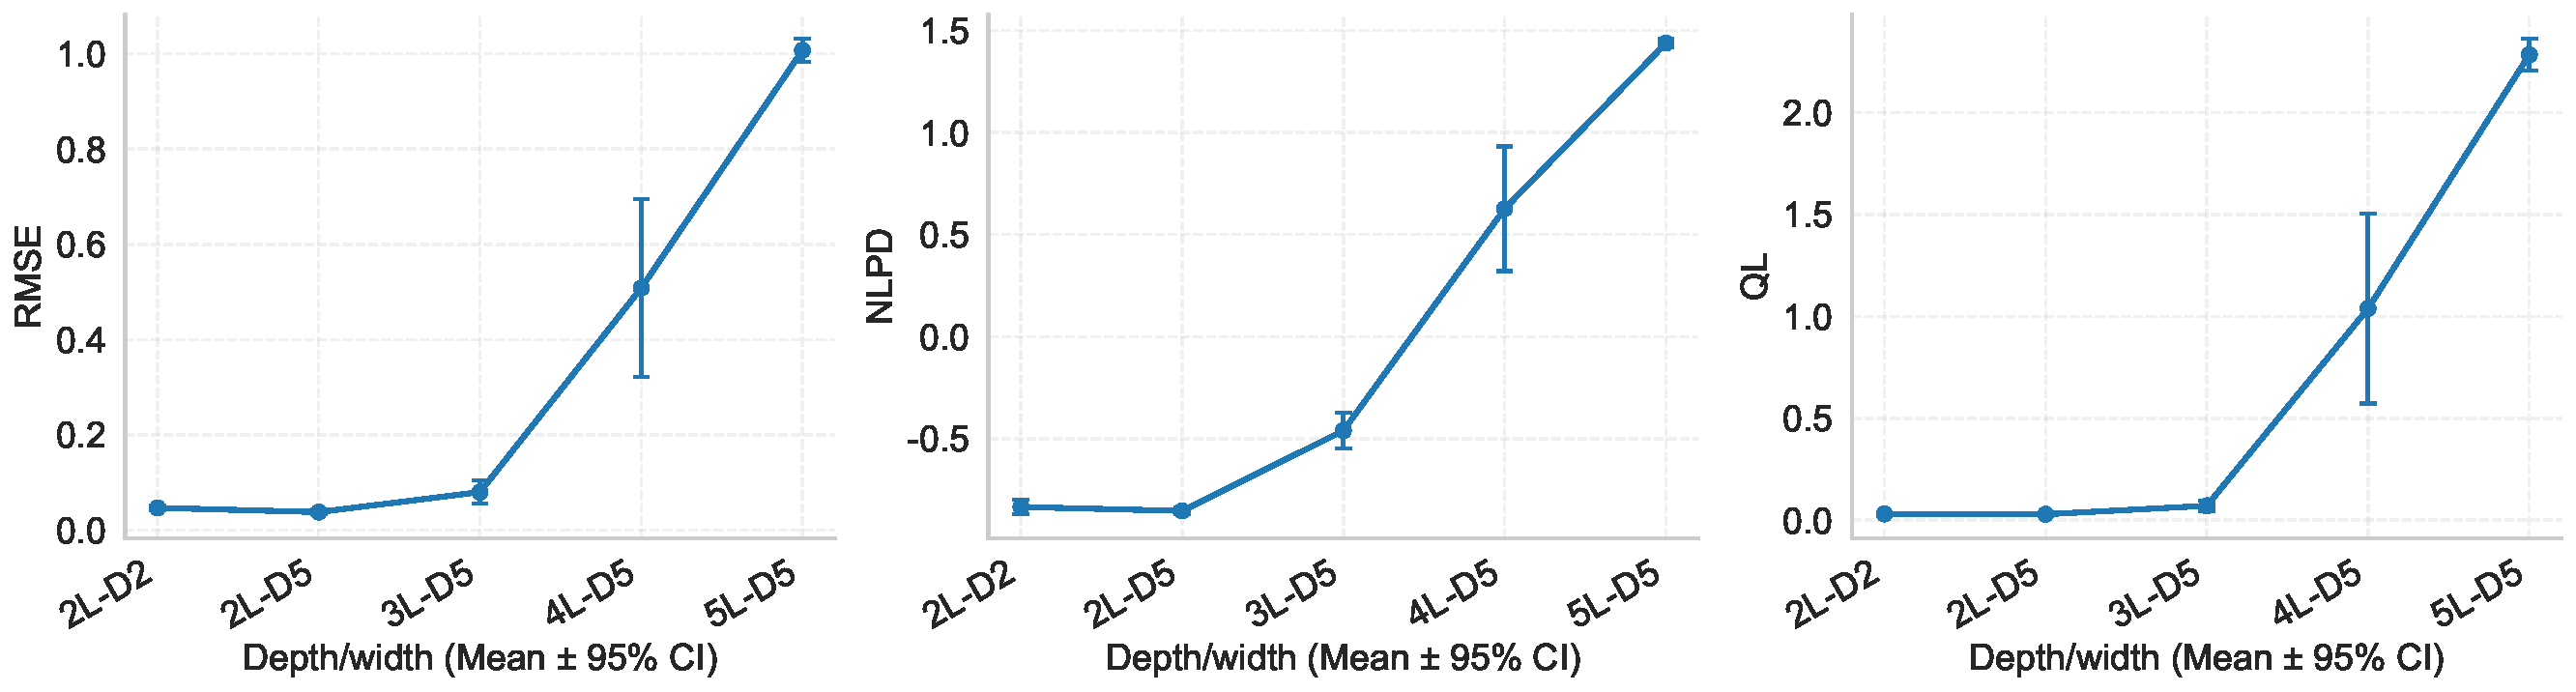
\includegraphics[width=\textwidth]{../mathexam/fig/sensitivity/depth_complexity/task1_metrics_errorbars.pdf}
			\caption{Task 1}
		\end{subfigure}

		\begin{subfigure}[b]{0.9\textwidth}
			\centering
			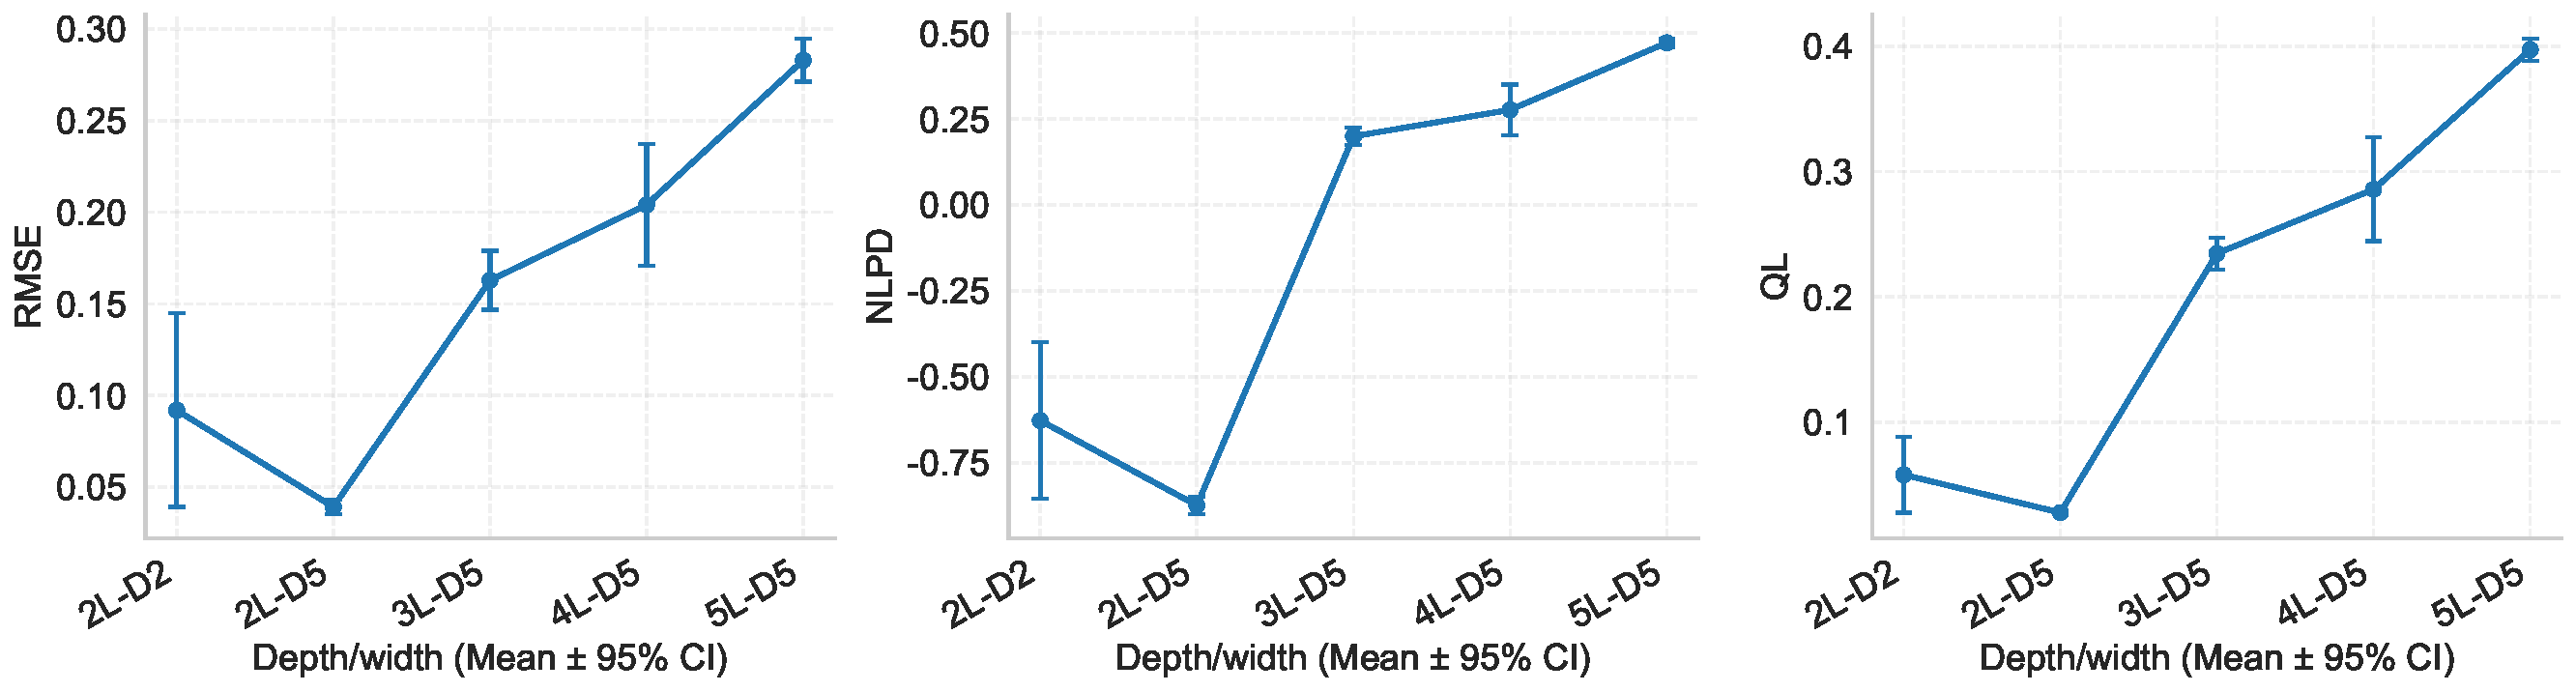
\includegraphics[width=\textwidth]{../mathexam/fig/sensitivity/depth_complexity/task2_metrics_errorbars.pdf}
			\caption{Task 2}
		\end{subfigure}

		\begin{subfigure}[b]{0.9\textwidth}
			\centering
			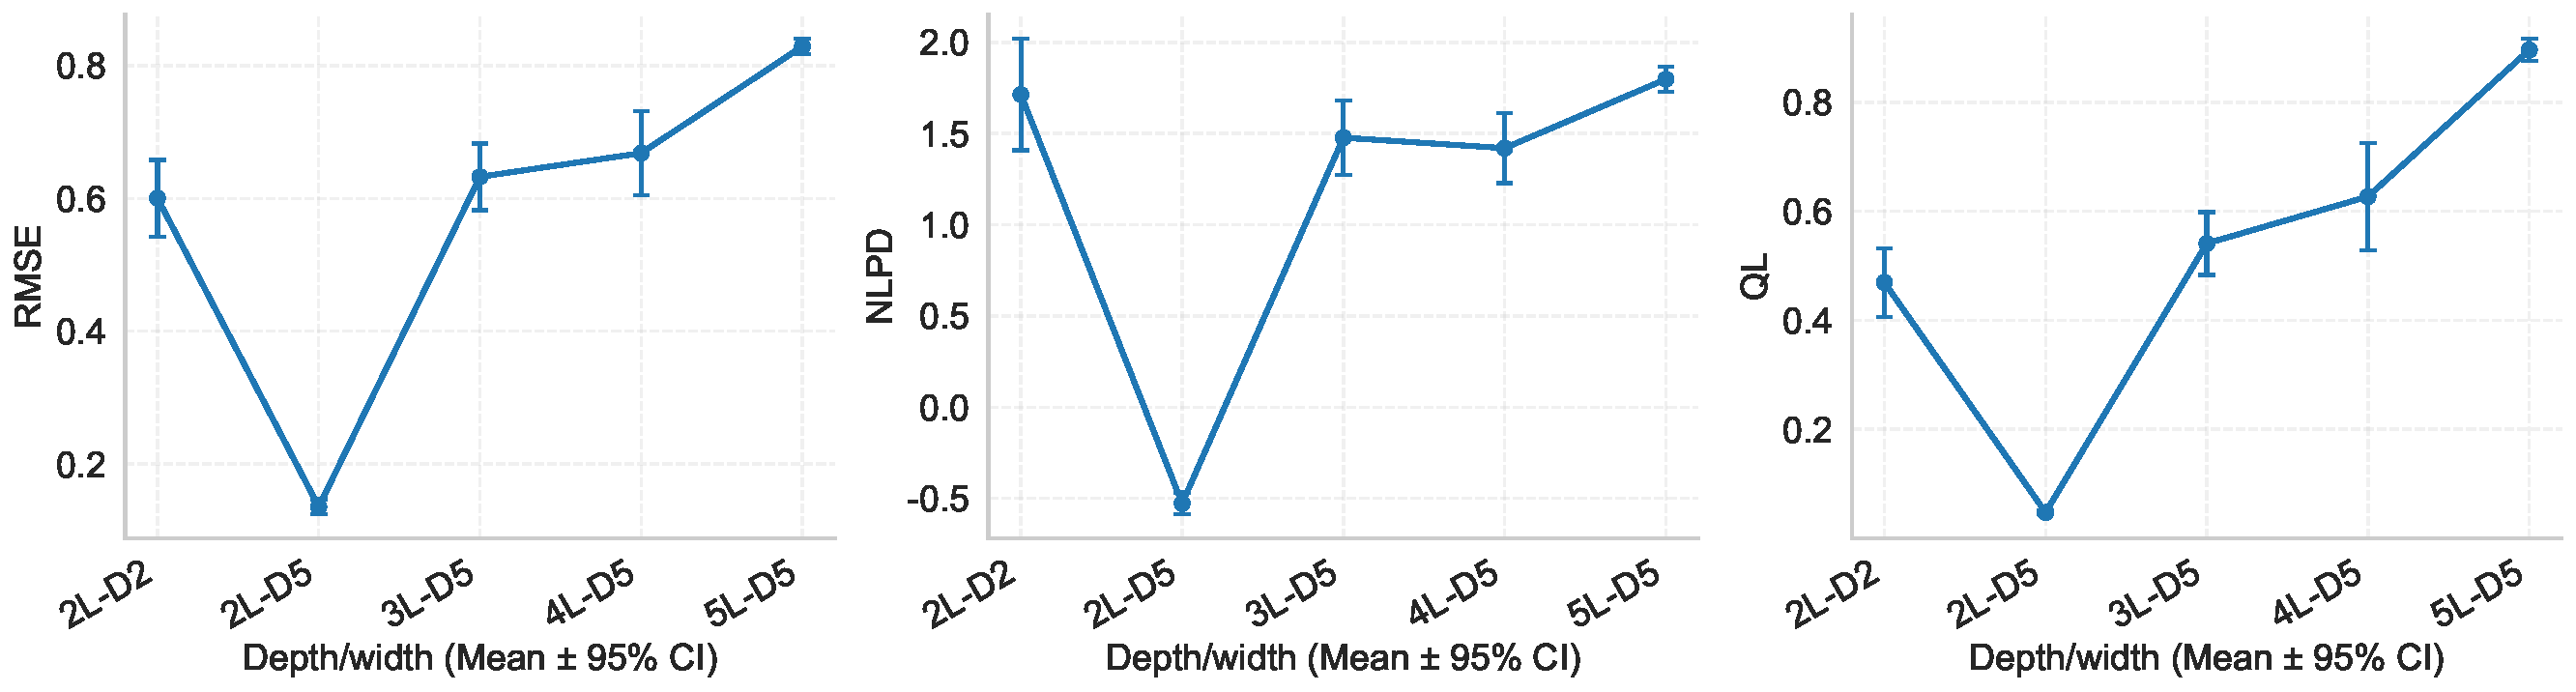
\includegraphics[width=\textwidth]{../mathexam/fig/sensitivity/depth_complexity/task3_metrics_errorbars.pdf}
			\caption{Task 3}
		\end{subfigure}
		\caption{Taskwise error-bar plots for depth and hidden-complexity sensitivity.}
		\caption*{深度与隐藏复杂度敏感性的分任务误差棒图。}
		\label{fig:depth_sensitivity}
	\end{figure}

	\subsection{Sample Size Sensitivity} \label{app:E3}
	The sample-size experiment highlights a strong finite-sample effect. Performance improves monotonically as the training size grows from 20 to 400. In particular, the average QL drops from 1.439658 at $n=20$ to \textbf{0.034749} at $n=400$, and the average RMSE drops from 0.592939 to \textbf{0.070777}. The pronounced gain from $n=200$ to $n=400$ further indicates that 400 samples are not excessive for this heterogeneous benchmark.

	样本量敏感性实验揭示了明显的有限样本效应。随着训练样本量从 20 增加到 400，性能呈单调改善趋势。特别是，平均 QL 从 $n=20$ 时的 1.439658 降至 $n=400$ 时的 \textbf{0.034749}，平均 RMSE 也从 0.592939 降至 \textbf{0.070777}。其中从 $n=200$ 到 $n=400$ 的显著跃迁进一步说明，对于该异质基准问题而言，400 个样本并不冗余。

	\begin{table}[htbp]
		\centering
		\caption{Average sensitivity summary for training sample size.}
		\caption*{训练样本量的平均敏感性汇总。}
		\label{tab:sample_sensitivity_avg}
		\begin{tabular}{lccc}
			\toprule
			Condition & Avg. RMSE & Avg. NLPD & Avg. QL \\
			\midrule
			$n=20$ & 0.592939 & 1.128905 & 1.439658 \\
			$n=50$ & 0.444696 & 0.992585 & 1.129003 \\
			$n=100$ & 0.403108 & 0.950088 & 1.033113 \\
			$n=200$ & 0.200731 & 0.304830 & 0.285129 \\
			$n=400$ & \textbf{0.070777} & \textbf{-0.751240} & \textbf{0.034749} \\
			\bottomrule
		\end{tabular}
	\end{table}

	\begin{figure}[htbp]
		\centering
		\begin{subfigure}[b]{0.9\textwidth}
			\centering
			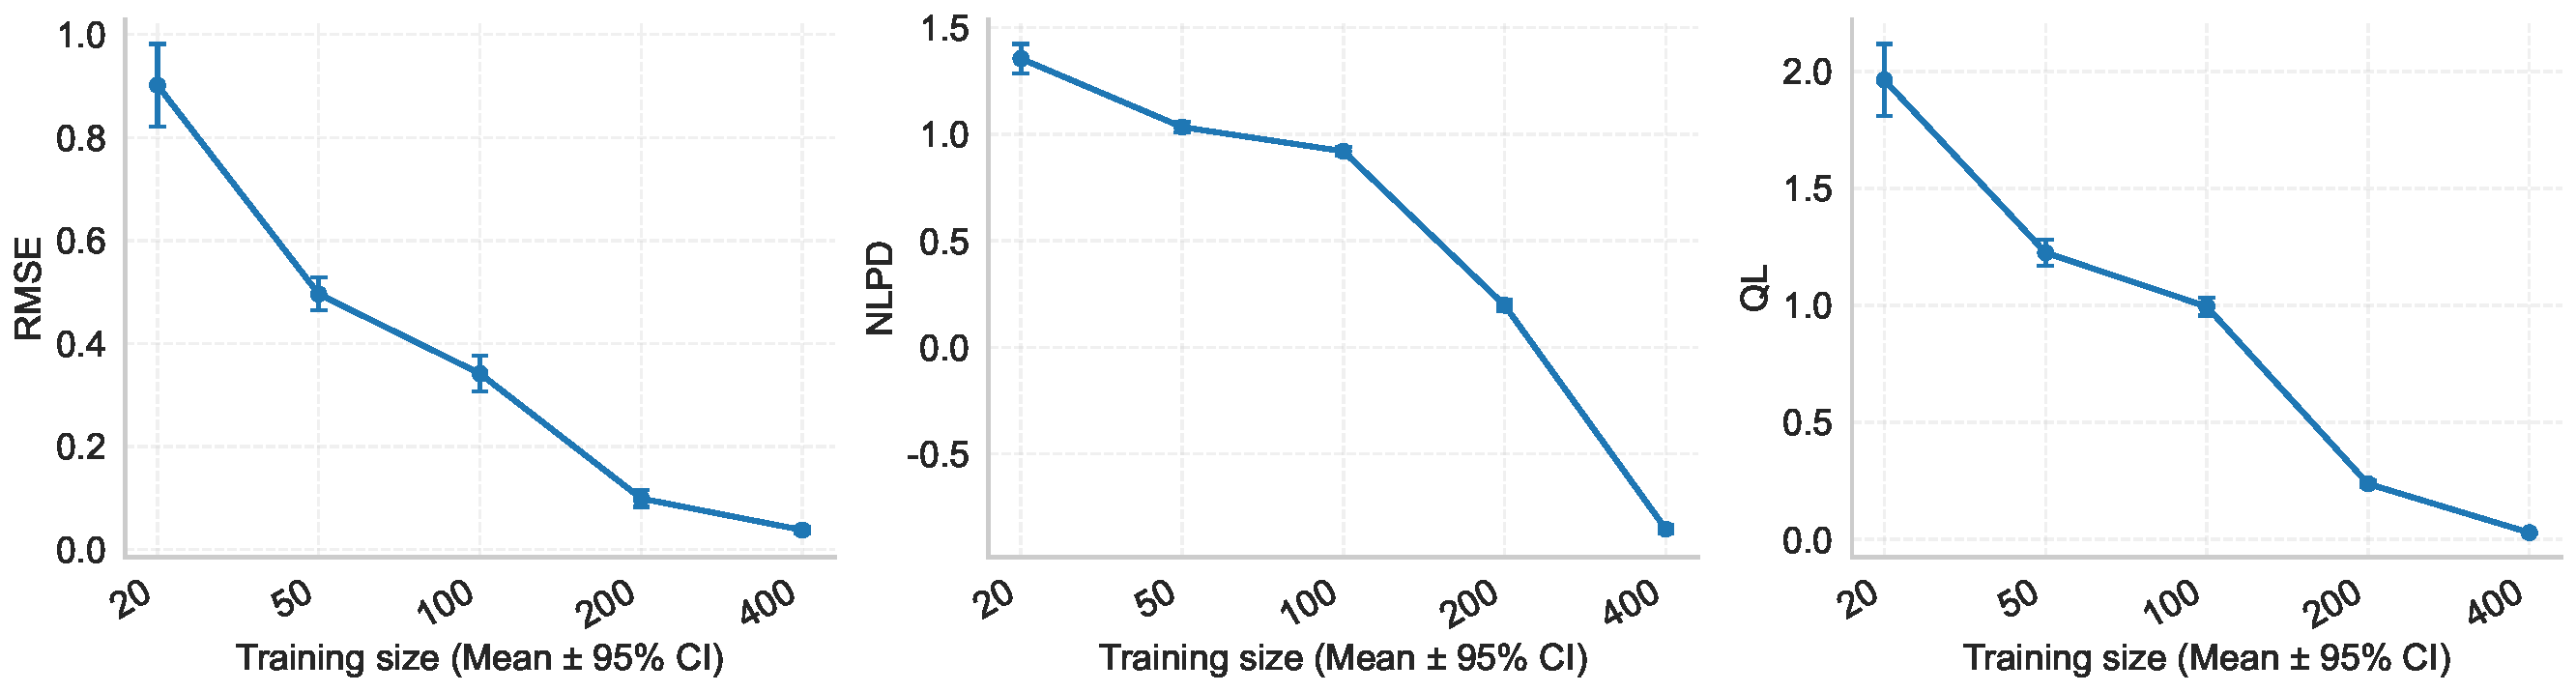
\includegraphics[width=\textwidth]{../mathexam/fig/sensitivity/sample_size/task1_metrics_errorbars.pdf}
			\caption{Task 1}
		\end{subfigure}

		\begin{subfigure}[b]{0.9\textwidth}
			\centering
			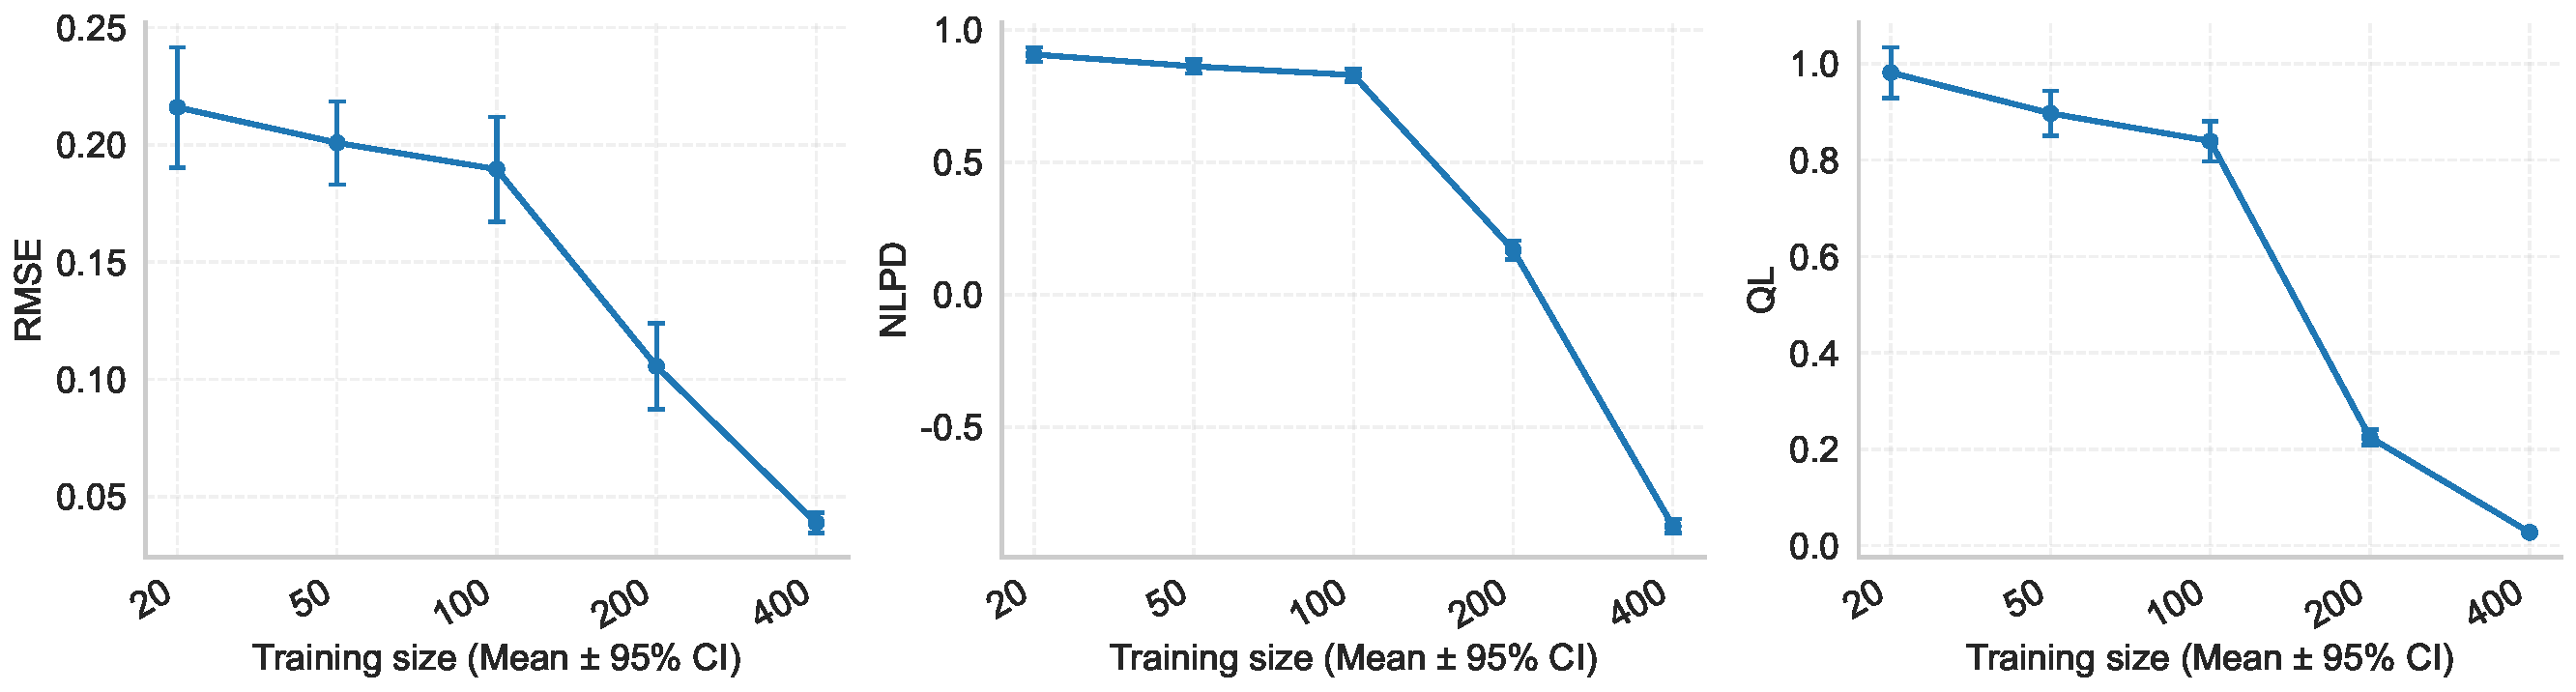
\includegraphics[width=\textwidth]{../mathexam/fig/sensitivity/sample_size/task2_metrics_errorbars.pdf}
			\caption{Task 2}
		\end{subfigure}

		\begin{subfigure}[b]{0.9\textwidth}
			\centering
			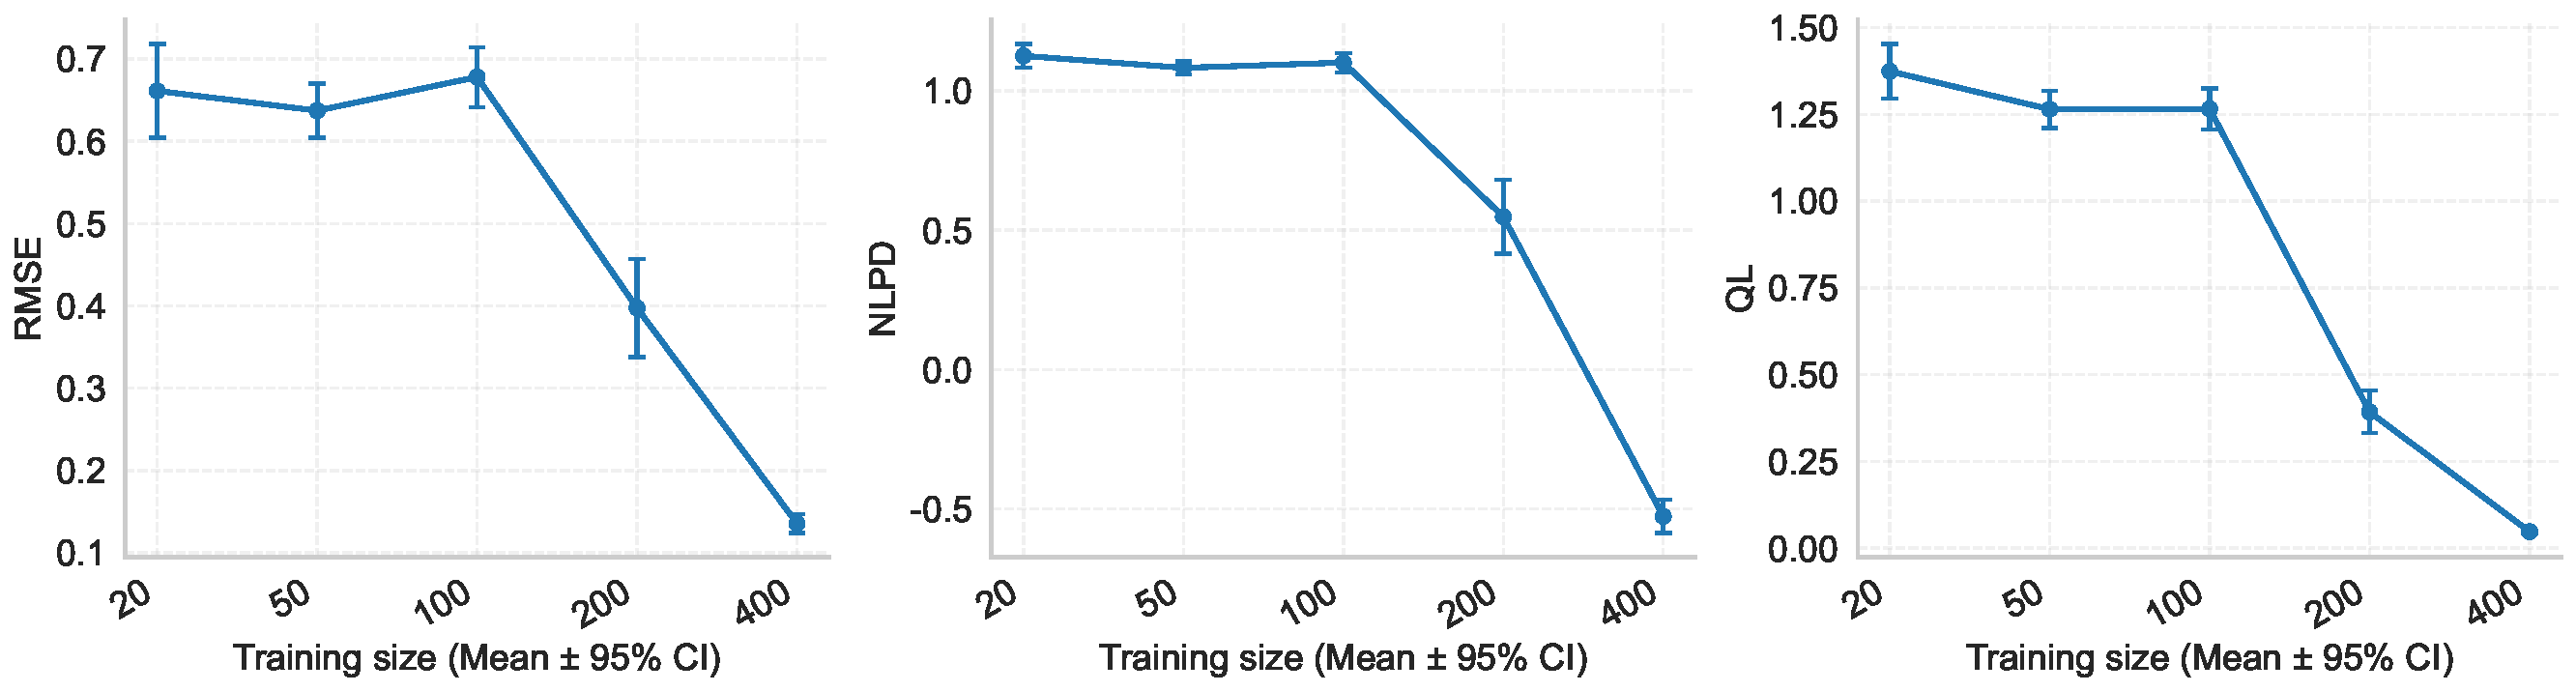
\includegraphics[width=\textwidth]{../mathexam/fig/sensitivity/sample_size/task3_metrics_errorbars.pdf}
			\caption{Task 3}
		\end{subfigure}
		\caption{Taskwise error-bar plots for sample-size sensitivity.}
		\caption*{训练样本量敏感性的分任务误差棒图。}
		\label{fig:sample_sensitivity}
	\end{figure}



	\newpage
	\section{Wall-clock Training Time and Time Complexity} \label{app:F}
	\resetappendixcounters % [#1]

	This appendix reports the detailed wall-clock training time and asymptotic time-complexity order of the Gaussian process surrogate methods evaluated in Section~4.2 of the main paper. All methods are trained for $500$ epochs on the OFDM dataset with $N=400$ training samples, $B=128$, $H=5$, $M=128$, $T=3$ and $L=3$, on a single workstation equipped with an NVIDIA RTX~2060 GPU, PyTorch~2.11+cu130 and Python~3.10. Table~\ref{tab:training_time_appendix} aggregates the total wall-clock time, the per-epoch time, the trainable-parameter count, and the asymptotic per-epoch order for each method.

	本附录给出正文 Section~4.2 中各高斯过程代理方法的 wall-clock 训练耗时与渐近时间复杂度。所有方法在 OFDM 数据集上训练 $500$ epochs，使用 $N=400$ 训练样本、$B=128$、$H=5$、$M=128$、$T=3$、$L=3$，硬件为一块 NVIDIA RTX~2060 GPU，软件栈为 PyTorch~2.11+cu130、Python~3.10。Table~\ref{tab:training_time_appendix} 汇总各方法的总耗时、单 epoch 耗时、可训练参数量以及单 epoch 的渐近阶。

	\begin{table}[!h]
		\centering
		\caption{Wall-clock training time of all Gaussian process surrogate methods on the OFDM dataset ($500$ epochs, NVIDIA RTX~2060, PyTorch~2.11+cu130).}
		\caption*{在 OFDM 数据集上各高斯过程代理方法的 wall-clock 训练耗时（$500$ epochs，NVIDIA RTX~2060，PyTorch~2.11+cu130）。}
		\label{tab:training_time_appendix}
		\begin{tabular*}{\textwidth}{@{\extracolsep{\fill}}lcccc}
			\toprule
			\textbf{Method} & \textbf{Total (s)} & \textbf{s/epoch} & \textbf{Params (K)} & \textbf{Asymptotic order} \\
			\midrule
			DA-DGP            & $397.79$ & $0.7956$ & $136.6$ & $\mathcal{O}(4\,E\lceil N/B\rceil(H+T)(BM^{2}\!+\!M^{3}))$\\
			\textcolor{red}{T-Atten}    & $387.78$ & $0.7756$ & $136.6$ & $\mathcal{O}(4\,E\lceil N/B\rceil(H+T)(BM^{2}\!+\!M^{3}))$\\% [#7]
			MGDA              & $164.87$ & $0.3297$ & $136.6$ & $\mathcal{O}(T\,E\lceil N/B\rceil(H+T)(BM^{2}\!+\!M^{3}))$\\
			Indep-DGP         & $163.40$ & $0.3268$ & $306.9$ & $\mathcal{O}(T\,E\lceil N/B\rceil(H+T)(BM^{2}\!+\!M^{3}))$\\
			DWA               & $109.25$ & $0.2185$ & $136.6$ & $\mathcal{O}(E\lceil N/B\rceil(H+T)(BM^{2}\!+\!M^{3}))$\\
			LMC-DGP           & $103.35$ & $0.2067$ & $136.7$ & $\mathcal{O}(E\lceil N/B\rceil(H+L)(BM^{2}\!+\!M^{3}))$\\
			Equal             & $100.57$ & $0.2011$ & $136.6$ & $\mathcal{O}(E\lceil N/B\rceil(H+T)(BM^{2}\!+\!M^{3}))$\\
			Pure DGP          & $\phantom{0}99.56$ & $0.1991$ & $136.6$ & $\mathcal{O}(E\lceil N/B\rceil(H+T)(BM^{2}\!+\!M^{3}))$\\
			UW                & $\phantom{0}96.04$ & $0.1921$ & $136.6$ & $\mathcal{O}(E\lceil N/B\rceil(H+T)(BM^{2}\!+\!M^{3}))$\\
			Indep-HetGP       & $\phantom{00}10.51$ & $0.0210$ & $0.021$ & $\mathcal{O}(E\,T\,N^{3})$\\
			\bottomrule
		\end{tabular*}
	\end{table}

	The constant factor in the per-epoch order of DA-DGP and \textcolor{red}{T-Atten} arises from the inner virtual update, the unrolled validation backward, and two finite-difference Hessian--vector evaluations introduced by the bilevel optimisation; the gradient-balancing baseline (MGDA) and the independent-task baseline (Indep-DGP) instead scale linearly in the number of tasks $T$. The heteroscedastic exact GP (Indep-HetGP) bypasses the variational machinery and is dominated by the dense $N\times N$ Cholesky factorisation, which remains affordable because $N=400$ is small. These numbers verify that the additional wall-clock overhead of DA-DGP is a small constant factor amortised over a single training pass, in exchange for the robust Pareto frontier reported in Table~7 of the main paper.% [#7]

	DA-DGP 与 \textcolor{red}{T-Atten} 的单 epoch 阶中的常数因子源自 bilevel 优化引入的内层虚拟更新、验证 unrolled 反向传播以及两次 finite-difference Hessian--vector 近似；梯度均衡基线（MGDA）和独立任务基线（Indep-DGP）则随任务数 $T$ 线性增长。异方差 exact GP（Indep-HetGP）不经过变分机制，其代价由 $N\times N$ Cholesky 分解主导，因 $N=400$ 较小而仍可接受。综上，DA-DGP 多出的 wall-clock 开销只是一次性训练中的小常数因子，所换得的是正文 Table~7 中的鲁棒 Pareto 前沿。% [#7]

	\subsection{\textcolor{red}{Robust Pareto Indicator Settings}} \label{app:F1}% [#4]

	\textcolor{red}{For reproducibility of the AHP-weighted TOPSIS ranking in Table~7 of the main paper, the nine robust Pareto indicators are treated as follows. The benefit-type indicators are \#P, \#GP, GC, $\mathrm{HV}_{\mathrm{n}}$, and HVR, whereas the cost-type indicators are IGD, IGD$^{+}$, spacing, and closest-ideal distance. The raw AHP weights assigned to these indicators are $[6,3,3,1,6,1,6,1,6]$, respectively, and are normalized to sum to one before TOPSIS aggregation. This setting gives higher emphasis to local-front density, hypervolume ratio, IGD$^{+}$, and closest-ideal distance while retaining the remaining indicators as supporting evidence, so the final $C_i$ rank should be read as an integrated robust-frontier assessment rather than a claim of dominance on every single metric.}% [#4]

	\textcolor{red}{为便于复核正文 Table~7 的 AHP 加权 TOPSIS 排名，九个鲁棒 Pareto 指标按如下方向处理：\#P、\#GP、GC、$\mathrm{HV}_{\mathrm{n}}$ 和 HVR 为收益型指标，IGD、IGD$^{+}$、spacing 与 closest-ideal distance 为成本型指标。对应的 AHP 原始权重依次为 $[6,3,3,1,6,1,6,1,6]$，并在 TOPSIS 聚合前归一化为和为一。该设定对局部前沿密度、超体积比、IGD$^{+}$ 和最近理想点距离赋予更高权重，同时保留其余指标作为支撑证据，因此最终 $C_i$ 排名应理解为综合鲁棒前沿评价，而非声称某一方法在每个单项指标上均逐项支配。}% [#4]

	\newpage
\begin{thebibliography}{99}

	% 注意：\bibitem 后面的 [Titsias(2009)] 是必须的，natbib 靠它来生成 (Author, Year)
	\bibitem[Titsias(2009)]{titsias2009variational}
	Titsias, M. (2009).
	Variational Learning of Inducing Variables in Sparse Gaussian Processes.
	\textit{Artificial Intelligence and Statistics (AISTATS), PMLR}, 5, 567--574.

	% 注意：\bibitem 后面的 [Knoblauch et~al.(2019)] 是必须的
	\bibitem[Knoblauch et~al.(2019)]{knoblauch2019generalized}
	Knoblauch, J., Jewson, J., \& Damoulas, T. (2019).
	Generalized Variational Inference: Three arguments for deriving new Posteriors.
	\textit{arXiv preprint arXiv:1904.02063}.

\end{thebibliography}

























\end{document}
